\section{QSAES21}

\begin{frame}{QSAES21\footfullcite{Jang}}
\begin{tabular}{cl}  
         \begin{tabular}{c}
            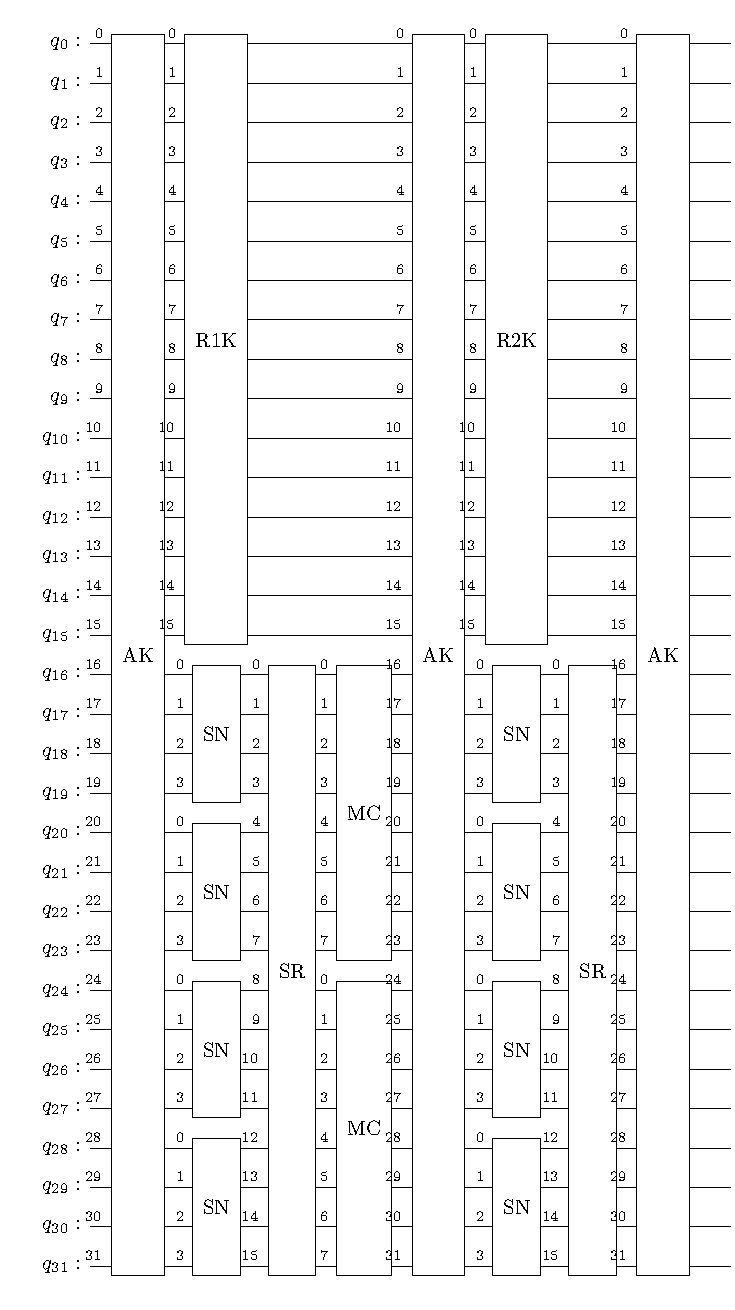
\includegraphics[width=0.4\linewidth]{saes21/saes.pdf}
           \end{tabular}
           & \begin{tabular}{l}
             \parbox{0.5\linewidth}{%  change the parbox width as appropiate
             \begin{itemize}
                 \item Only uses 32 qubits and no ancilla qubits.
                 \pause
                 \item The top 16 qubits are used for storing the master key and for the process of key expansion.
                 \pause
                 \item The bottom 16 qubits are used for storing plaintext, round operations, and outputting ciphertext.
             \end{itemize}
    }
         \end{tabular}  \\
\end{tabular}
\end{frame}
\begin{frame}{Sub Nibbles}
    \begin{itemize}
        \item Unlike \cite{Almazrooie}\footfullcite{Almazrooie} which uses 16 qubits (4 input, 4 output, and 8 ancillae) for Sbox computation, \cite{Jang}\footfullcite{Jang} uses only 4 qubits using LIGHTER-R tool \cite{LighterR}\footfullcite{LighterR}.
        \pause
        \item Output is permuted so we need SWAP gates (Not measured in quantum resources).
    \end{itemize}
    
    \begin{figure}[h!]
        \centering
        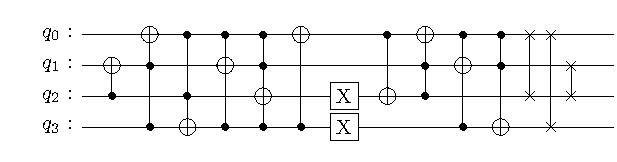
\includegraphics[width=1\linewidth]{saes21/sbox.pdf}
        \caption{Sbox}
        \label{fig:sb21}
    \end{figure}
\end{frame}
\begin{frame}{Shift Rows and Mix Column}
\begin{itemize}
    \item Shift rows operation using swap gates only whereas \cite{Almazrooie}\footfullcite{Almazrooie} used extra qubits for that with additional CNOT gates.
    \pause
    \item Compared to \cite{Almazrooie}, the authors use less number of qubits but require SWAP gates to get the correct result.
\end{itemize}
\begin{figure}[h!]
    \centering
    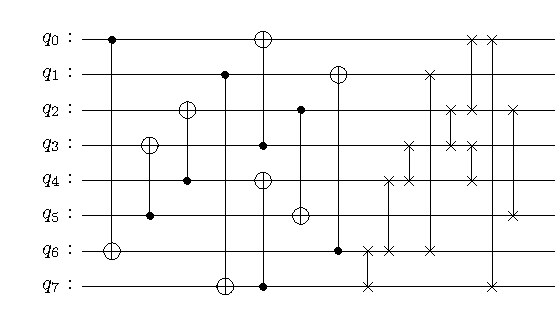
\includegraphics[width=0.7\linewidth]{saes21/mc.pdf}
    \caption{Mix column}
    \label{fig:mc21}
\end{figure}
\end{frame}
\begin{frame}{Key Exapansion}
    Round keys are generated on the fly.
    \begin{figure}[h!]
    \centering
    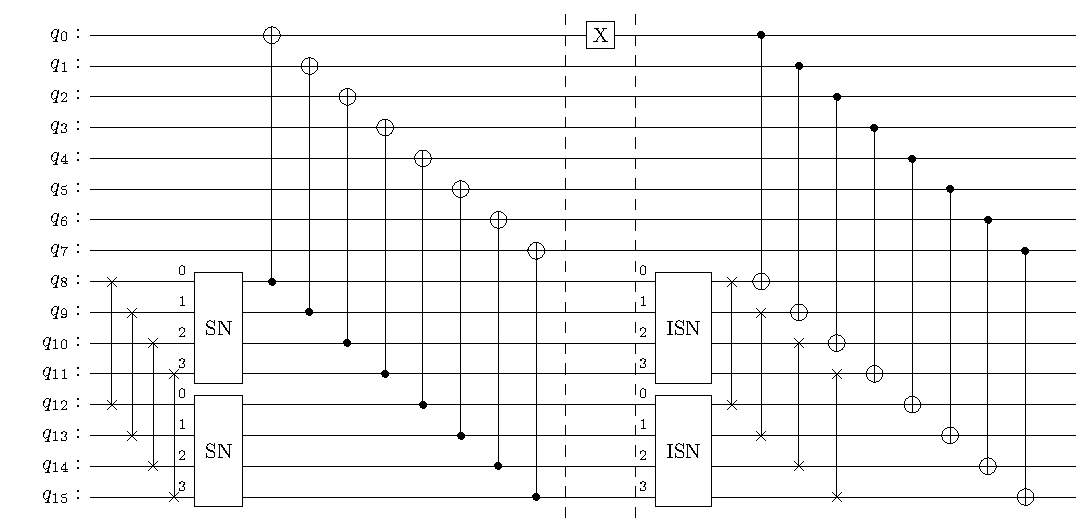
\includegraphics[width=0.8\linewidth]{saes21/r1k.pdf}
    \caption{Round key 1}
    \label{fig:rk121}
\end{figure}
\pause
\begin{itemize}
    \item Swap and substitution of $B_1$ then xor it with $B_0$.
    \pause
    \item Add Round constant (10000000).
    \pause
    \item Now the first 8 qubits hold $B_2$. To get $B_3$, we need to xor $B_1$ and $B_2$ but $B_1$ is lost.
    \pause
    \item Inverse swap and substitution on the lower 8 qubits to get back $B_1$. Xor $B_2$ with $B_1$ to get $B_3$.
    
\end{itemize}
\end{frame}
\begin{frame}{Grover's Attack}
    \begin{itemize}
        \item Expt1:  verified the encryption process on IBMQ QASM Simulator \cite{IBMQ}\footfullcite{IBMQ}.
        \pause
        \item Expt2 : Superpostion of all keys on IBM's Statevector simulator for 4000 shots.
    \end{itemize}
    \begin{figure}[h!]
    \centering
    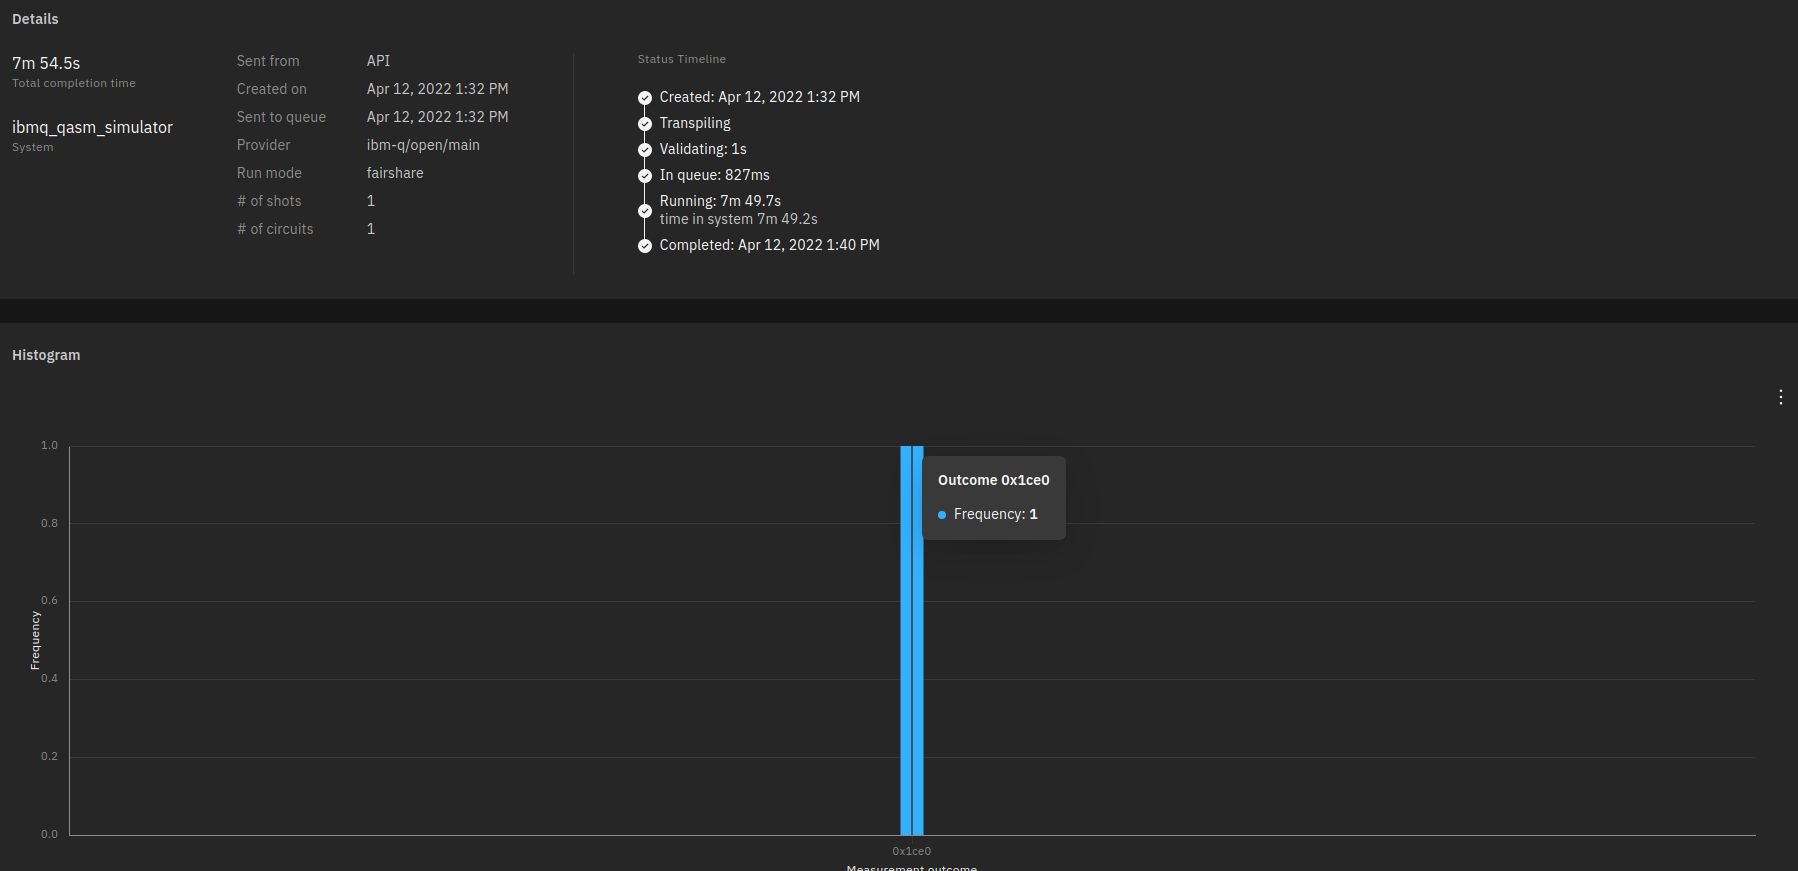
\includegraphics[width=0.7\linewidth]{saes21/encryption.png}
    \caption{Output of encryption of plaintext 0110 1111 0110 1011 with key 1010 0111 0011 1011}
    \label{fig:expt1res}
\end{figure}
Output is $0x1ce0$ in hexadecimal, which in binary is 0001 1100 1110 0000 which is the reverse of the ciphertext.
\end{frame}
\begin{frame}{Grover's Attack Contd.}
    \begin{figure}[h!]
    \centering
    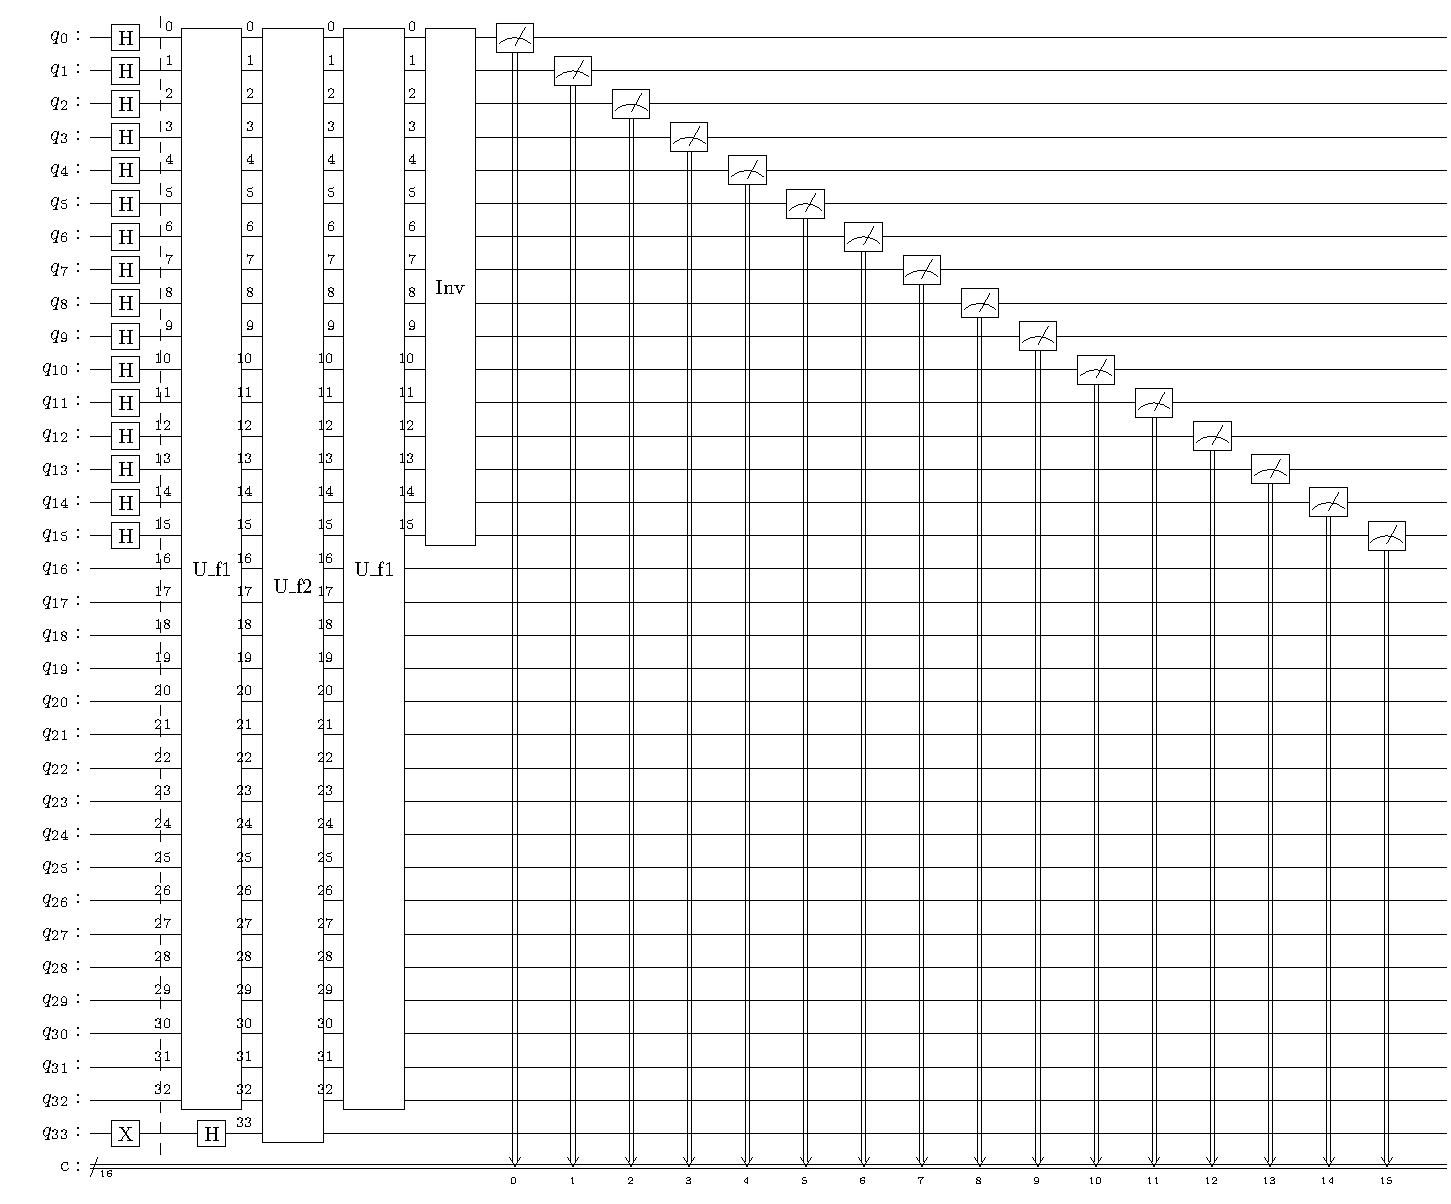
\includegraphics[width=0.8\linewidth]{saes21/grover-coupling-1-iter.pdf}
    \caption{Grover's Attack for unique key with r = 2 (1 iteration)}
    \label{fig:grov21u}
\end{figure}
\end{frame}
\begin{frame}{Cost Estimates}
    \begin{center}
\begin{table}[h!]
    \centering
    \begin{tabular}{ |c|c|c|c|c|c|c| } 
     \hline
       & Qubits & X & CX & CCX & Ancilla \\ \hline
     Key expansion & 32 & 10& 568 & 192 & 8 \\ \hline
     Encryption & 32 & 16 & 512 & 384 & - \\ \hline
     Total & 64 & 26 & 1080 & 576 & 8 \\ \hline
     Key expansion & 16 & 19& 56 & 48 & - \\ \hline
     Encryption & 16 & 16 & 88 & 48 & - \\ \hline
     Total & 32 & 35 & 144 & 96 & - \\ \hline
     My Code & 32 & 35 & 144 & 96 & - \\ \hline
    \end{tabular}
    \caption{Comparison of cost for QSAES18\cite{Almazrooie} and QSAES21\cite{Jang} }
    \label{tab:cost21}
\end{table}
\end{center}
\pause
Cost was heavily reduced due to optimizations in Sbox, key expansion, and mix columns circuit. Cost of Grover's Attack is :
\begin{equation*}
    2\times 2\times \frac{\pi}{4}\sqrt{2^{16}}
\end{equation*}
\end{frame}